\iffalse
\documentclass[12pt]{article}
\usepackage{graphicx}
%\documentclass[journal,12pt,twocolumn]{IEEEtran}
\usepackage[none]{hyphenat}
\usepackage{graphicx}
\usepackage{listings}
\usepackage[english]{babel}
\usepackage{graphicx}
\usepackage{caption} 
\usepackage{hyperref}
\usepackage{booktabs}
\usepackage{commath}
\usepackage{gensymb}
\usepackage{array}
\usepackage{amsmath}   % for having text in math mode
\usepackage{listings}
\lstset{
  frame=single,
  breaklines=true
}
  
%Following 2 lines were added to remove the blank page at the beginning
\usepackage{atbegshi}% http://ctan.org/pkg/atbegshi
\AtBeginDocument{\AtBeginShipoutNext{\AtBeginShipoutDiscard}}
%


%New macro definitions
\newcommand{\mydet}[1]{\ensuremath{\begin{vmatrix}#1\end{vmatrix}}}
\providecommand{\brak}[1]{\ensuremath{\left(#1\right)}}
\providecommand{\norm}[1]{\left\lVert#1\right\rVert}
\newcommand{\solution}{\noindent \textbf{Solution: }}
\newcommand{\myvec}[1]{\ensuremath{\begin{pmatrix}#1\end{pmatrix}}}
\let\vec\mathbf


\begin{document}
\begin{center}
\title{\textbf{Straight Lines}}
\date{\vspace{-5ex}} %Not to print date automatically
\maketitle
\end{center}
\setcounter{page}{1}
\section{11$^{th}$ Maths - Exercise 10.3.8}

\begin{enumerate}
\section{Solution}Given equation expressed as  
\begin{align}
	\vec{n}^{\top}\vec{x}=c
\end{align}
\fi
The given line parameters are
\begin{align}
		\vec{n} = \myvec{1\\-7},\, c=-5 
\end{align}
yielding
\begin{align}
	\vec{m} =\myvec{7 \\ 1}
\end{align}
The perpendicular passes through
\begin{align}
	\vec{A} &=\myvec{3\\0}
\end{align}
Hence, the desired equation is
		\begin{align}
			\myvec{7 & 1}\brak{\vec{x}-\myvec{3\\0}} &=0\\
		\implies 	\myvec{7 & 1}\vec{x} &= 21
		\end{align}
		See Fig. 
\ref{fig:chapters/11/10/3/8/Fig1}.
		\begin{figure}[!h]
\begin{center}
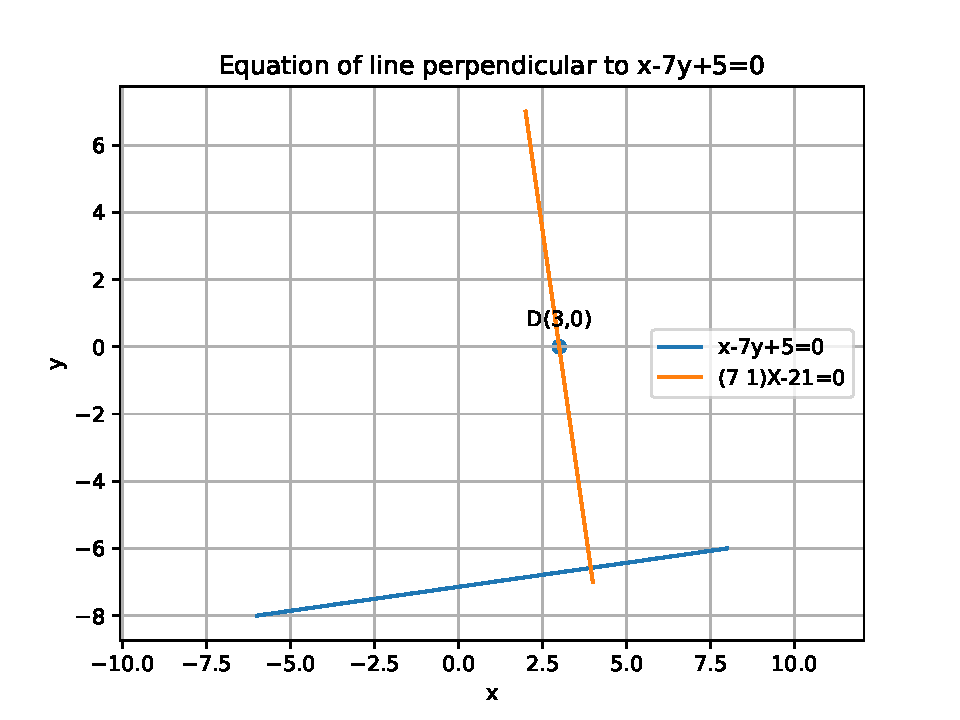
\includegraphics[width=\columnwidth]{chapters/11/10/3/8/figs/fig.pdf}
\end{center}
\caption{}
\label{fig:chapters/11/10/3/8/Fig1}
\end{figure}
